\documentclass[answers]{exam}

\usepackage{amsmath}
\usepackage{amssymb}
\usepackage{geometry}
\usepackage{venndiagram}
\usepackage{graphics}
\usepackage{graphicx}
\usepackage{tikz}
\usepackage{listings}
\usepackage{hyperref}
\usepackage{float}
\usepackage{xcolor}

\lstset{
    language=Matlab,
    basicstyle=\ttfamily\small,
    breaklines=true,
    keywordstyle=\color{blue},
    commentstyle=\color{green},
    stringstyle=\color{purple},
    numbers=left,
    numberstyle=\tiny\color{gray},
    stepnumber=1,
    showspaces=false,
    showstringspaces=false,
    frame=single,
    postbreak=\mbox{\textcolor{red}{$\hookrightarrow$}\space},
}

\geometry{
    bottom=2cm, % Adjust this value as needed to leave space for the answer boxes
}

% Header and footer.
\pagestyle{headandfoot}
\runningheadrule
\runningfootrule
\runningheader{EE/CE 468/468 Mobile Robotics}{Homework 4}{Fall 2023}
\runningfooter{}{Page \thepage\ of \numpages}{}
\firstpageheader{}{}{}

\boxedpoints
\printanswers

\newcommand{\uvec}[1]{\boldsymbol{\hat{\textbf{#1}}}}
\newcommand\union\cup
\newcommand\inter\cap
\newcommand\ul\underline
\newcommand\ol\overline

\title{Assignment 4\\ EE/CE 468/468 Mobile Robotics\\ Habib University -- Fall 2023}
\author{Ali Asghar Yousuf \\ Muhammad Azeem Haider }
\date{\today}

\begin{document}
\maketitle

\begin{questions}
    \question[25]
    \textbf{Sensor Model}. Assume that you're building a sensor model for the robot used in the previous homework assignment that was equipped with a sensor capable of measuring the distance
    and bearing to landmarks. Furthermore, assume that this sensor is also capable of identifying
    the landmarks, so that when you receive a range and bearing measurement you know which
    landmark it corresponds to.

    A sensor measurement $z = (r, \theta)T$ is composed of the measured distance,
    $r$, and the measured bearing, $\theta$, to the landmark $l$. Both the range
    and the bearing measurements are subject to zero-mean Gaussian noise with
    variances $\sigma_r^2$ and $\sigma_\theta^2$, respectively. The range and the
    bearing measurements are independent of each other.

    Design a sensor model $p(z|x, l)$ for this type of sensor and explain it.

    \begin{solution}
        The sensor model $p(z|x, l)$ can be designed as follows:

        \[
            p(z|x, l) = p(r, \theta|x, l) = p(r|x, l) \cdot p(\theta|x, l)
        \]

        where $p(r|x, l)$ represents the probability distribution of the range
        measurement given the robot's state $x$ and the landmark $l$, and $p(\theta|x,
            l)$ represents the probability distribution of the bearing measurement given
        the robot's state $x$ and the landmark $l$.

        Since both the range and bearing measurements are subject to zero-mean Gaussian
        noise, we can model $p(r|x, l)$ and $p(\theta|x, l)$ as Gaussian distributions.
        Specifically, we can use the following equations:

        \[
            p(r|x, l) = \frac{1}{\sqrt{2\pi\sigma_r^2}} \exp\left(-\frac{(r - \hat{r})^2}{2\sigma_r^2}\right)
        \]

        \[
            p(\theta|x, l) = \frac{1}{\sqrt{2\pi\sigma_\theta^2}} \exp\left(-\frac{(\theta - \hat{\theta})^2}{2\sigma_\theta^2}\right)
        \]

        where $\hat{r}$ and $\hat{\theta}$ are the expected range and bearing
        measurements, respectively, based on the robot's state $x$ and the landmark
        $l$.

        By combining these equations, we can obtain the sensor model $p(z|x, l)$ for
        the given sensor.

        \[
            p(z | x, l) = \frac{1}{2\pi\sigma_r\sigma_\theta} \exp\left(-\frac{(r - \hat{r})^2}{2\sigma_r^2} - \frac{(\theta - \hat{\theta})^2}{2\sigma_\theta^2}\right)
        \]

        We can write $r - \hat{r}$ and $\theta - \hat{\theta}$ as $\Delta r$ and
        $\Delta \theta$, respectively, and take the negative in the exponent common to
        obtain the final expression:

        \[
            p(z | x, l) = \frac{1}{2\pi\sigma_r\sigma_\theta} \exp\left[- \left(\frac{(\Delta r)^2}{2\sigma_r^2} + \frac{(\Delta \theta)^2}{2\sigma_\theta^2}\right)\right]
        \]
    \end{solution}

    \question[25]
    \textbf{Grid-based Occupancy Mapping}. In this problem, you'll implement occupancy grid mapping
    for a simple one-dimensional environment, spanning from left to right, e.g. imagine one long
    lane (1D), using a sequence of measurements from a range sensor. The length of the map or
    this lane is 2 meters. Divide the map into cells of size 10 cm. Choose a representative point
    (coordinate) for each cell according to some rule and state your rule. Our robot is placed in
    the left-most cell and has a range sensor mounted on it that is oriented towards the right, or
    towards the lane. The robot does not move while building this map.

    Assume a very simple model for the sensor: every grid cell with a distance from
    the robot that is smaller than the measured distance is assumed to be occupied
    with probability $0.3$. Every cell behind the measured distance is occupied
    with probability $0.6$. Every cell located more than $20$ cm behind the
    measured distance should not be updated.

    Assume that we have no prior information about the occupancy of any cell. The
    robot receives the following sequence of measurements, from its range sensor,
    at different time steps: $\{101, 82, 91, 112, 99, 151, 96, 85, 99, 105\}$.

    Using MATLAB, find the belief of the map incorporating all the measurements.
    Plot the probability values of each cell against your chosen representative
    points to obtain a PMF. Based on the obtained belief, draw the map.

    \begin{solution}
        \begin{figure}[H] % Example image
            \centering
            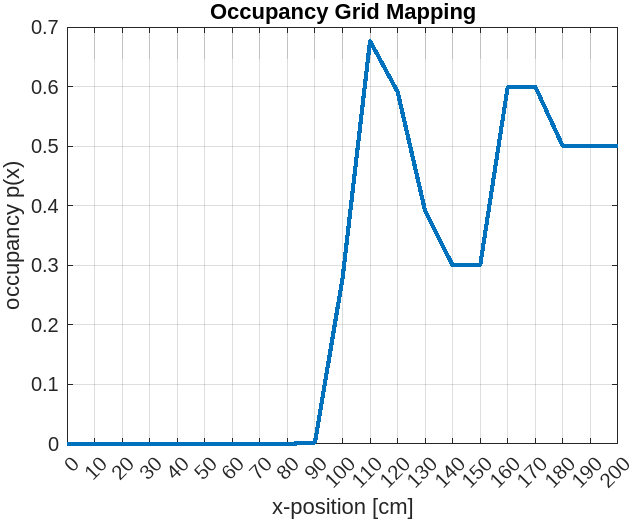
\includegraphics[width=0.5\textwidth]{Q2PMF.png} % Image path and size
            \caption{Probability Mass Function (PMF) of the occupancy grid map}
            \label{fig:image1} % Label for referencing the figure
        \end{figure}

        \begin{figure}[H] % Example image
            \centering
            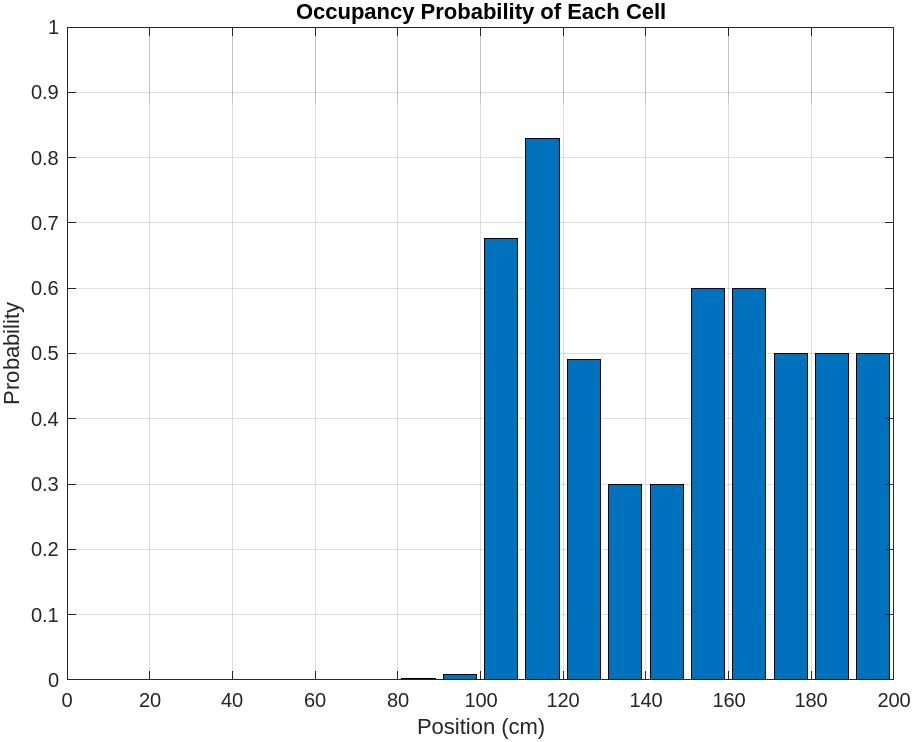
\includegraphics[width=0.5\textwidth]{Q2PMF2.png} % Image path and size
            \caption{Probability Mass Function (PMF) of the occupancy grid map}
            \label{fig:image1} % Label for referencing the figure
        \end{figure}

        We can compare the two graphs to see that the probability of the cells are same
        when viewed as discretized cells or continuous.

        \begin{lstlisting}[language=Matlab, caption=Occupancy Grid Mapping, label={lst:code}]
function occupancy_grid_mapping()
    % We will first define our sensor model in which we will add conditions depending on the distane of the cell from the robot
    function log_odds = inv_sensor_model(z, c)
        if c > z + 20
            % If the measurement is beyong 20 cm, we will not update the cell as per the instructions
            log_odds = 0;
        elseif c > z
            % If the cell is behind the measured distance, it is occupied with probability 0.6
            log_odds = log(0.6 / (1 - 0.6));
        else
            % If the cell distance is smaller than the measured distance, it is occupied with probability 0.3
            log_odds = log(0.3 / (1 - 0.3));
        end
    end

    % We divide our path of 2 meter into grids of 10 cm
    c = 0:10:200;

    % Map belief
    logodds = zeros(1, length(c));

    % Measurements in cm
    meas = [101, 82, 91, 112, 99, 151, 96, 85, 99, 105];

    prior = log(0.5 / (1 - 0.5));
    disp(['prior:', num2str(prior)]);

    % Update map with each measurement
    for i = 1:length(meas)
        % Update each cell
        for j = 1:length(c)
            % Update log-odds using the inverse sensor model
            logodds(j) = logodds(j) - prior + inv_sensor_model(meas(i), c(j));
        end
    end

    % Converting the logodds function to probability 
    m = 1 - 1 ./ (1 + exp(logodds));

    figure;
    plot(c, m, 'LineWidth', 2);
    xticks(0:10:200);
    xlabel('x-position [cm]');
    ylabel('occupancy p(x)');
    title('Occupancy Grid Mapping');
    grid on;
end     
        \end{lstlisting}

        \textbf{Explanation of the graph:} The x-axis in the graph shows the position of the robot along the 2 meter line that is provided in the question. The line is divided into twenty distinct cells of size 10 cm as described in the question. The peaks in the graph signify occupancy of the cells and that is our condition 2 and 3, reflecting the sensor model's assignment of a 0.3 probability to cells within the measured distance and a 0.6 probability to cells just behind the measured distance up to 20 cm. The flat line in the start of the graph tells is that the cells were never updated because they were 20 cm behind any measurement. Finally the represetative point is the center of each cell that is 5, 15, 25, 35, 45, and so on cm on the 2 meter line.

    \end{solution}

    \question[25]
    In Problem 4 of the last homework assignment, you used EKF for landmark-based localization, where the line features in the environment played the role of landmarks. In this problem, you'll solve the same localization problem using particle filter, or in other words apply Monte Carlo Localization.
    \begin{parts}
        \part Code
        \begin{solution}
            Similarly to the previous homework, we will be using most of the same code for this question. The main
            difference in implementing the particle filter is that we will be using a set of particles to represent the
            robot's belief instead of a Gaussian distribution. We will also be using the same sensor model as the
            previous homework.

            We implemented a \texttt{generateParticles} function to initialize the
            particles. The function is shown in Listing \ref{lst:code1}. The function takes
            in the number of particles to be generated and the map as parameters. It then
            generates the particles randomly on the map and returns the particles.

            \begin{lstlisting}[language=Matlab, caption=Generate Particles, label={lst:code1}]
function particles = generateParticles(numParticles, map)
    angles = map(1,:);
    M = map(2,:);

    left_max = max(M(angles == 0));
    right_max = max(M(angles == pi));
    up_max = max(M(angles == pi/2));
    down_max = max(M(angles == -pi/2));

    particles = zeros(4, numParticles);
    particles(1,:) = unifrnd(-left_max, right_max, 1, numParticles);
    particles(2,:) = unifrnd(-down_max, up_max, 1, numParticles);
    particles(3,:) = unifrnd(0, 2*pi, 1, numParticles);
    particles(4,:) = ones(1, numParticles);
end
            \end{lstlisting}

            We modified the \texttt{filterStep} function from the previous homework to
            implement the particle filter. The modified function is shown in Listing
            \ref{lst:code2}.
            \begin{lstlisting}[language=Matlab, caption=Filter Step, label={lst:code2}]
function [updated_particles, P_posterior] = filterStep(particles, P, u, Q, Z, R, M, g, b)
    N = size(particles,2);
    X_new = particles(1:3, :);
    W_new = particles(end, :);

    for i = 1:N
        X_prev = particles(1:3,i);
        [X_bar,Fx, Fu]= odometry(X_prev, u, b);
        X_new(1:3,i)=X_bar;
        [z_, H_seq, R_seq, Associated_landmark] = MCL_association(X_new, P(:,i:i+2), Z, R, M, g);
        if sum(Associated_landmark) > 0
            % If a correspondence was found
            for j = 1:size(z_,2)
                % The loop is only for when there are multiple measurements
                pdf = measurementProbability(z_(:,j), R_seq(:,:,j), M(:,j), X_bar);
                W_new(i) = pdf*W_new;
            end
        % Update the Covariance matrix P
        P(:,i:i+2) = update_P(P(:,i:i+2), H_seq, Fu, Fx, Q, R);
        end
    end
    % Normalize
    W_new = W_new/sum(W_new);
    updated_particles = resampleParticles(X_new, W_new, N);
    P_posterior = P;
end
            
            \end{lstlisting}
            We implemented some helper functions as well to make the code more readable
            including \texttt{odometry}, \texttt{resampleParticles},
            \texttt{measurementProbability}, \texttt{MCL\_association}, and
            \texttt{update\_P}. The code for these functions is shown in Listings
            \ref{lst:code3}, \ref{lst:code4}, \ref{lst:code5}, \ref{lst:code6} and
            \ref{lst:code7}, respectively.

            \begin{lstlisting}[language=Matlab, caption=Odometry, label={lst:code3}]
function [x_bar, Fx, Fu] = odometry(x, u, b)
    theta = x(3,1);
    x_bar = zeros(3,1);
    x_bar(1,1) = x(1,1) + (u(1,1) + u(2,1))/2 * cos(theta);
    x_bar(2,1) = x(2,1) + (u(1,1) + u(2,1))/2 * sin(theta);
    x_bar(3,1) = x(3,1) + (-u(1,1) + u(2,1))/b;
    Fx = [
        1 0 -sin(theta);
        0 1 cos(theta);
        0 0 1
        ];
    Fu = [
        cos(theta)/2 cos(theta)/2;
        sin(theta)/2 sin(theta)/2;
        -1/b 1/b
        ];
end
            \end{lstlisting}

            \begin{lstlisting}[language=Matlab, caption=Resample Particles, label={lst:code4}]
function updated_particles = resampleParticles(X_new, W_new, N)
    % The w array needs to be normalized
    index = [];
    cdf = zeros(1,N);
    % create CDF
    cdf(1) = w(1);
    for i = 2:size(w,2)
        cdf( i) = cdf( i-1) + w(i);
    end

    u = unifrnd(0,1/N);
    for j = 1:N
        i = 1;
        while u > cdf(:, i)
            i = i + 1;
        end
        index = [index i];
        u = u + 1/N;
    end
    X_new = X(:,index);

    particles = [X_new;
                ones(1, N)];
    % disp("This is it")
    % particles
end
            \end{lstlisting}

            \begin{lstlisting}[language=Matlab, caption=Measurement Probability, label={lst:code5}]
function pdf = measurementProbability(z, R, M, X)
% The function returns the weight of the i_th particle
    mu_z = [angdiff(M(1,1) - X(3,1));
            M(2,1) - ( X(1,1)*cos(M(1,1)) + X(2,1)*sin(M(1,1)));
            ]; %This is the expected value of z given x_bar
    pdf = mvnpdf(z,mu_z,R);
end
              \end{lstlisting}

            \begin{lstlisting}[language=Matlab, caption=Associate Landmarks, label={lst:code6}]
function [z_, H_seq, R_seq, Associated_landmarks] = MCL_association(x, P, Z, R, M, g)
    % [v, H, R] = associateMeasurements(x, P, Z, R, M, g) returns a set of
    % innovation vectors and associated jacobians and measurement covariances
    % by matching line features by Mahalanobis distance.
    % v: Matrix of innovations for the selected measurements.
    % H: Corresponding Jacobians.
    % R: Covariance matrices of selected measurements.


    % Make use of the measurementFunction.m to find the predicted measurements.


    first_entry = true;
    H_seq = [];
    R_seq = [];
    z_ = [];
    Associated_landmarks = zeros(size(M,2)) ;%Associated landmark index
    for i = 1:size(Z,2)
        min_d = inf;
        min_m = 0;
        min_Hx = 0;
        found = false;
        for j = 1:size(M,2)
            [h, H_x] = measurementFunction(x, M(:,j));
            v_ijt = Z(:,i) - h;
            % h_size = size(H_x)
            % P_size = size(P)
            % R_size = size(R)
            % RR = size(R(:,:,i))
            % bruh = H_x*P*H_x'+R(:,:,i)
            
            % R(:,:,i)
            Sigma_ijINt = H_x*P*H_x'+R(:,:,i);
            d_curr = transpose(v_ijt)*Sigma_ijINt^(-1)*v_ijt;
            if d_curr <= min_d
                found = true;
                min_d = d_curr;
                min_m = i;
                min_Hx = H_x;
                Associated_landmarks(j) = 1;
            end
        end
        if found == true
            if first_entry == true && min_d <= g^2
                % disp("A Correspondence is Found")
                first_entry = false;
                z_ = [z_ Z(:, i)];
                H_seq = min_Hx;
                R_seq = R(:,:,min_m);
            elseif min_d <= g^2
                % disp("A Correspondence is Found")
                z_ = [z_ Z(:, i)];
                H_seq(end+1:end+2,:) = min_Hx;
                R_seq(end+1:end+2,end+1:end+2) = R(:,:,min_m);
            end
        end
    end
end
            \end{lstlisting}

            \begin{lstlisting}[language=Matlab, caption=Update Particles, label={lst:code7}]
function [P] = updateP(P, H, Fu, Fx, Q, R)
    % size_H = size(H)
    % H
    % size_P = size(P)
    P_BAR = Fx*P*Fx'+Fu*Q*Fu';
    PINt = H*P_BAR*H' + R;
    Kk = P_BAR*H'*(PINt)^(-1);
    P = P_BAR - Kk*PINt*Kk'; 
end
            \end{lstlisting}

            We are using the same \texttt{measurementFunction} as the previous homework.
        \end{solution}
        \part Results
        \part Discussion
    \end{parts}

    \question[(Bonus) 20]
    This \href{https://www.mathworks.com/help/nav/ug/landmark-slam-using-apriltag-markers.html}{linked Mathworks example} uses pose graph and factor graphs for SLAM, given odom-
    etry data and measurement data from April Tag markers being used as landmarks. You'll
    instead implement the EKF-SLAM algorithm on the same data, to obtain the locations of all
    landmarks and the trajectory of the robot.

    \begin{solution}
    \end{solution}

    \question[20]
    Answer the following questions individually:
    \begin{parts}
        \part How many hours did each of you spend on this homework?
        \begin{solution}
            \subsection*{Ali Asghar Yousuf}
            7 hours
            \subsection*{Muhammad Azeem Haider}
            12 hours
        \end{solution}

        \part State each group member's specific contribution to this homework assignment.
        \begin{solution}
            We will be submitting question 3 later.
            \subsection*{Ali Asghar Yousuf}
            Question 1 and 3

            \subsection*{Muhammad Azeem Haider}
            Question 2 and 3
        \end{solution}

        \part Do you have any specific advice for students attempting this homework next year?
        \begin{solution}
            % TODO: Add advice
            \subsection*{Ali Asghar Yousuf}
            At this point of the semester, everything is starting to get a bit
            overwhelming. The best way to tackle this is to start early and not leave
            things for the last minute. I would also recommend to go through the slides and
            the book before starting the questions. This will help you understand the
            theory behind the questions and will make it easier to solve them.

            \subsection*{Muhammad Azeem Haider}
            Understanding the theory behind why things are happening is extremely important
            to make sure that these assignments are completed smoothly. I found myself
            stuck in my many questions previously, and in question 2 this time where I
            banged my head trying to fix the "code" only to realize the logic I applied was
            incorrect and it was all down to a lack of understanding of the question topic.
            As a result, it is absolutely imperative I feel like before starting questions,
            go through the instructor slides or the reference pages/sections in the
            respective book to build a stronger theoretical framework so when you're trying
            to complete the solution you are able to complete it smoothly.

        \end{solution}

        \part Provide a self-reflection in the form of a note or a concept map.
        \begin{solution}
            % TODO: Add self-reflection
            \subsection*{Ali Asghar Yousuf}
            Designing the sensor model was a bit tricky but I found the slides extremely
            helpful. I am also currently taking the course on Applied Stochastic Processes
            so the probability part was not that difficult for me. As for the 3rd question,
            it is still a work in progress. I understand the theory behind it but I am
            having trouble implementing it. I will try to complete it as soon as possible.

            \subsection*{Muhammad Azeem Haider}
            I attempted Question 2 and 3. While question 2 was seemingly easy, trying to
            figure out how to incorporate the measurements to get a belief was going to
            work. It took me some time and google searches to finally understand how I can
            get it to work. Implementing Monte Carlo Localization was especially a
            challenge when it came to question 3, the matrix dimension errors were
            persistent and I was not able to properly figure it out despite going through
            the book.

        \end{solution}
    \end{parts}
\end{questions}

\end{document}